% ============================================================
%  RELATÓRIO ACADÉMICO — SISTEMA DE ESTATÍSTICA DE LISTAS
%  Grupo 4 | Curso de Licenciatura em informatica | 2026
% ============================================================
\documentclass[12pt, a4paper, oneside]{report}

% ---------- Codificação e língua ----------
\usepackage[utf8]{inputenc}
\usepackage[T1]{fontenc}
\usepackage[portuguese]{babel}

% ---------- Geometria ----------
\usepackage[
  top=3cm, bottom=2.5cm,
  left=3cm, right=2.5cm,
  headheight=15pt
]{geometry}

% ---------- Tipografia ----------
\usepackage{lmodern}
\usepackage{microtype}
\usepackage{setspace}
\onehalfspacing

% ---------- Gráficos e cores ----------
\usepackage{graphicx}
\usepackage[dvipsnames,svgnames,x11names]{xcolor}
\usepackage{float}
\usepackage{subcaption}
\usepackage{caption}

% ---------- Tabelas ----------
\usepackage{longtable}
\usepackage{booktabs}
\usepackage{array}
\usepackage{multirow}

% ---------- Código-fonte ----------
\usepackage{listings}

% Estilo Haskell
\lstdefinestyle{haskell}{
  language=Haskell,
  basicstyle=\ttfamily\small,
  keywordstyle=\color{MidnightBlue}\bfseries,
  commentstyle=\color{OliveGreen}\itshape,
  stringstyle=\color{BrickRed},
  numberstyle=\tiny\color{gray},
  numbers=left,
  stepnumber=1,
  numbersep=8pt,
  frame=single,
  framesep=4pt,
  rulecolor=\color{gray!50},
  breaklines=true,
  showstringspaces=false,
  tabsize=4,
  captionpos=b,
  backgroundcolor=\color{gray!5},
}

% Estilo Bash/Terminal
\lstdefinestyle{bash}{
  language=bash,
  basicstyle=\ttfamily\small,
  keywordstyle=\color{DarkGreen}\bfseries,
  commentstyle=\color{gray}\itshape,
  numberstyle=\tiny\color{gray},
  numbers=left,
  stepnumber=1,
  numbersep=8pt,
  frame=single,
  framesep=4pt,
  rulecolor=\color{gray!50},
  breaklines=true,
  showstringspaces=false,
  tabsize=2,
  captionpos=b,
  backgroundcolor=\color{black!3},
  morekeywords={git, mkdir, cd, pwd, touch, ghc, ls},
}

\renewcommand{\lstlistingname}{Código}
\renewcommand{\lstlistlistingname}{Lista de Códigos}

% ---------- Hiperligações ----------
\usepackage[
  colorlinks=true,
  linkcolor=MidnightBlue,
  citecolor=OliveGreen,
  urlcolor=BrickRed,
  pdftitle={Relatório -- Sistema de Estatística de Listas em Haskell},
  pdfauthor={Grupo 4},
]{hyperref}

% ---------- Cabeçalhos e rodapés ----------
\usepackage{fancyhdr}
\pagestyle{fancy}
\fancyhf{}
\fancyhead[L]{\small\textit{Sistema de Estatística de Listas em Haskell}}
\fancyhead[R]{\small\textit{Grupo 4 -- 2026}}
\fancyfoot[C]{\thepage}
\renewcommand{\headrulewidth}{0.4pt}
\renewcommand{\footrulewidth}{0.2pt}

% ---------- TikZ ----------
\usepackage{tikz}
\usetikzlibrary{arrows.meta, positioning, shapes.geometric, calc}

% ---------- Índice e listas automáticas ----------
\usepackage{tocloft}
\setlength{\cftbeforetoctitleskip}{0pt}

% ---------- Outros ----------
\usepackage{amsmath}
\usepackage{amssymb}
\usepackage{enumitem}
\usepackage{indentfirst}
\usepackage{titlesec}
\usepackage{parskip}
\setlength{\parindent}{1.5cm}
\setlength{\parskip}{0.2cm}

% Formatação de títulos de capítulos
\titleformat{\chapter}[display]
  {\normalfont\huge\bfseries\color{MidnightBlue}}
  {\chaptertitlename\ \thechapter}{16pt}{\Huge}
\titlespacing*{\chapter}{0pt}{0pt}{20pt}

% Reformular \maketitle
\usepackage{titling}

% Tolerância a hbox ligeiramente largos (evita overfull warnings menores)
\hfuzz=30pt

% ============================================================
\begin{document}
% ============================================================

% ============================================================
%  CAPA -- Universidade Licungo
% ============================================================
\begin{titlepage}
\begin{center}

\vspace*{0.8cm}


\includegraphics[width=0.38\textwidth]{logo_licungo.png}

\vspace{0.7cm}

{\Large \bfseries UNIVERSIDADE LICUNGO}\\[0.15cm]
{\normalsize Faculdade de Ci\^{e}ncias e Tecnologias}\\[0.05cm]
{\normalsize Curso de Licenciatura em Inform\'{a}tica}

\vspace{1.4cm}

{\large \bfseries LABORAT\'{O}RIO 1}

\vspace{1.4cm}

{\LARGE \bfseries Sistema de Estat\'{i}stica de Listas em Haskell}\\[0.4cm]
{\normalsize utilizando Linux, Git e GitHub}

\vspace{1.8cm}

\begin{large}
\begin{tabular}{@{}rl@{}}
\textbf{Grupo:}    & Grupo 4 \\[0.35cm]
\textbf{Docente:}  & Daniel Gimo \\[0.35cm]
\multirow{4}{*}{\textbf{Estudantes:}}
  & Ac\'{a}cio Rombe Machica \\
  & Alberto Lucas Alface \\
  & Cl\'{a}udio Armando Cha\'{u}que \\
  & Pedro Francisco Antonio \\
\end{tabular}
\end{large}

\vfill

{\normalsize Beira, 10 de Julho de 2026}

\end{center}
\end{titlepage}

% ============================================================
%  FOLHA DE ROSTO (CONTRACAPA)
% ============================================================
\thispagestyle{empty}
\begin{center}

\vspace*{0.8cm}


\includegraphics[width=0.32\textwidth]{logo_licungo.png}

\vspace{0.6cm}

{\Large \bfseries UNIVERSIDADE LICUNGO}\\[0.15cm]
{\normalsize Faculdade de Ci\^{e}ncias e Tecnologias}\\[0.05cm]
{\normalsize Curso de Licenciatura em Inform\'{a}tica}

\vspace{1.2cm}

{\LARGE \bfseries Sistema de Estat\'{i}stica de Listas em Haskell}\\[0.2cm]
{\normalsize utilizando Linux, Git e GitHub}

\vspace{1.0cm}

\begin{flushleft}
\hspace{7.5cm}
\begin{minipage}{0.46\linewidth}
\normalsize
Trabalho pr\'{a}tico apresentado no \^{a}mbito da Cadeira de Laborat\'{o}rio 1, do Curso de Licenciatura em Inform\'{a}tica da Universidade Licungo, como requisito parcial de avalia\c{c}\~{a}o, sob orienta\c{c}\~{a}o do Docente Daniel Gimo.
\end{minipage}
\end{flushleft}

\vspace{1.0cm}

\begin{large}
\begin{tabular}{@{}rl@{}}
\textbf{Grupo:}    & Grupo 4 \\[0.3cm]
\textbf{Docente:}  & Daniel Gimo \\[0.3cm]
\multirow{4}{*}{\textbf{Estudantes:}}
  & Ac\'{a}cio Rombe Machica \\
  & Alberto Lucas Alface \\
  & Cl\'{a}udio Armando Cha\'{u}que \\
  & Pedro Francisco Antonio \\
\end{tabular}
\end{large}

\vfill

{\normalsize Beira, 10 de Julho de 2026}

\end{center}
\clearpage
% ============================================================
%  LISTAS AUTOMÁTICAS
% ============================================================
\pagestyle{fancy}
\tableofcontents
\clearpage

\listoffigures
\clearpage

\listoftables
\clearpage

\lstlistoflistings
\clearpage

% ============================================================
%  CAPÍTULO 1 — INTRODUÇÃO
% ============================================================
\chapter{Introdução}

\section{Contextualização}

No panorama tecnológico contemporâneo, as competências de programação representam um pilar estruturante da formação de informaticos em qualquer ramo da área técnica. No contexto específico, a capacidade de desenvolver software para processamento de dados, desenvolvimento de sistemas web, apps nativos e embarcados constitui um diferencial competitivo de elevado valor.

\subsection{Importância da Programação Funcional}

A programação funcional representa um paradigma de desenvolvimento de software que se distingue fundamentalmente da programação imperativa tradicional. Enquanto a programação imperativa descreve \textit{como} um programa deve executar uma sequência de comandos que alteram o estado do sistema, a programação funcional concentra-se em \textit{o que} o programa deve computar, expressando a solução através de funções matemáticas puras.

As vantagens do paradigma funcional incluem a eliminação de efeitos colaterais indesejados (\textit{side effects}), a facilidade de raciocínio formal sobre o código, a maior facilidade de teste e depuração, e a adequação natural ao processamento paralelo. Em contextos de informatica, onde a correção e a previsibilidade do software são críticas, o paradigma funcional oferece garantias formais que os paradigmas imperativos não conseguem fornecer de forma nativa.

\subsection{Importância do Haskell}

Haskell é uma linguagem de programação funcional pura, com tipagem estática forte e avaliação preguiçosa (\textit{lazy evaluation}). Foi concebida em 1990 por um comité de investigadores com o objetivo de criar uma linguagem funcional padrão para investigação e ensino. Ao longo das décadas seguintes, Haskell evoluiu para uma plataforma robusta, amplamente utilizada tanto na academia como na indústria, em domínios que vão desde sistemas financeiros até compiladores e verificação formal de software.

A relevância académica do Haskell reside na sua capacidade de promover uma compreensão profunda dos fundamentos matemáticos da computação, nomeadamente teoria de tipos, cálculo lambda e álgebra de tipos. O estudo de Haskell desenvolve nos estudantes um raciocínio computacional mais rigoroso e transferível para qualquer outra linguagem ou paradigma.

\subsection{Importância do Git}

O Git é um sistema de controlo de versões distribuído, criado por Linus Torvalds em 2005, originalmente para gerir o desenvolvimento do kernel Linux. Tornou-se o padrão de facto para controlo de versões em projetos de software de qualquer dimensão, sendo utilizado por praticamente todas as organizações tecnológicas do mundo.

O Git permite que os programadores registem o histórico completo das alterações efectuadas num projeto, revertam para versões anteriores em caso de erro, trabalhem em paralelo em diferentes funcionalidades através de ramificações (\textit{branches}), e integrem contribuições de múltiplos colaboradores de forma organizada. No contexto deste projeto, o Git foi utilizado como ferramenta essencial de documentação do processo de desenvolvimento incremental.

\subsection{Importância do Linux no Desenvolvimento de Software}

O Linux é um sistema operativo de código aberto, baseado no kernel criado por Linus Torvalds em 1991. Representa o ambiente de desenvolvimento preferencial para a grande maioria dos programadores profissionais, servidores, supercomputadores e sistemas embarcados a nível mundial.

Para o desenvolvimento em Haskell, o Linux oferece um ambiente nativo superior, com instalação simplificada do compilador GHC (\textit{Glasgow Haskell Compiler}), integração directa com o terminal e as ferramentas de desenvolvimento, e ausência de camadas de abstração que em outros sistemas operativos podem complicar o fluxo de trabalho. O domínio do terminal Linux é, portanto, uma competência indispensável para qualquer engenheiro de software moderno.

\section{Problema}

O presente trabalho surge da necessidade de processamento eficiente de listas numéricas para extração de métricas estatísticas fundamentais. Em muitos contextos de informatica, é necessário analisar conjuntos de dados numéricos para obter rapidamente informações como a soma total, a média, os valores extremos e a dimensão do conjunto. A implementação de um sistema que automatize este processo, com verificação rigorosa de tipos e comportamento previsível, constitui o problema central que este projeto procura resolver.

\section{Objetivo Geral}

Desenvolver um sistema de estatística de listas em Haskell, executado em ambiente Linux, com controlo de versões gerido pelo Git e hospedagem no GitHub, capaz de processar listas de números fornecidas pelo utilizador e calcular automaticamente as métricas estatísticas fundamentais.

\section{Objetivos Específicos}

\begin{enumerate}[label=\arabic*.]
  \item Ler e processar listas de números fornecidas pelo utilizador através do terminal Linux;
  \item Implementar a função de cálculo da soma de todos os elementos da lista;
  \item Implementar a função de cálculo da média aritmética da lista;
  \item Implementar a função de determinação do maior valor da lista;
  \item Implementar a função de determinação do menor valor da lista;
  \item Implementar a função de contagem do número de elementos da lista;
  \item Utilizar o Git para controlo e documentação do processo de desenvolvimento;
  \item Utilizar o GitHub para hospedagem remota e gestão do repositório;
  \item Demonstrar o uso de \textit{branches} para desenvolvimento paralelo e incremental.
\end{enumerate}

\section{Metodologia}

O desenvolvimento do projeto seguiu uma metodologia de desenvolvimento incremental baseada no modelo de ramificações do Git. O processo foi organizado em quatro etapas sequenciais, cada uma implementada numa \textit{branch} dedicada, sendo a integração realizada através de operações de \textit{merge} na \textit{branch} principal (\texttt{master}).

O fluxo de trabalho adoptado pode ser descrito como: (1) criação da estrutura base na \textit{branch} principal; (2) desenvolvimento incremental de funcionalidades em \textit{branches} dedicadas; (3) integração de cada \textit{branch} na \textit{branch} principal após conclusão e teste; (4) realização de testes manuais com múltiplas entradas para validação do sistema. Este modelo garante um histórico de commits limpo, onde cada \textit{commit} corresponde a um estado funcional do sistema.

% ============================================================
%  CAPÍTULO 2 — FUNDAMENTAÇÃO TEÓRICA
% ============================================================
\chapter{Fundamentação Teórica}

\section{Haskell}

\subsection{História}

Haskell foi criada em 1990 como resultado do trabalho do \textit{Haskell Committee}, um grupo de investigadores de universidades norte-americanas e europeias que reconheceram a necessidade de uma linguagem funcional padrão que pudesse servir de base para investigação académica. O nome foi atribuído em homenagem ao lógico Haskell Curry, cujo trabalho em lógica combinatória e cálculo lambda constitui um dos fundamentos matemáticos da programação funcional.

Desde a versão inicial Haskell 1.0 de 1990, a linguagem evoluiu significativamente, tendo o padrão Haskell 98 e posteriormente Haskell 2010 consolidado a especificação moderna da linguagem. O compilador GHC (\textit{Glasgow Haskell Compiler}) tornou-se a implementação de referência, oferecendo desempenho comparável a linguagens compiladas como C e C++ em muitos cenários.

\subsection{Características Fundamentais}

Haskell distingue-se de outras linguagens de programação por um conjunto de características únicas:

\begin{itemize}
  \item \textbf{Pureza funcional:} todas as funções em Haskell são matemática e formalmente puras, no sentido em que a mesma entrada produz sempre o mesmo resultado, sem efeitos secundários no estado do sistema;
  \item \textbf{Tipagem estática forte:} o sistema de tipos de Haskell verifica a correção do programa em tempo de compilação, prevenindo uma vasta classe de erros em tempo de execução;
  \item \textbf{Avaliação preguiçosa (\textit{lazy evaluation}):} as expressões em Haskell só são avaliadas quando os seus resultados são necessários, permitindo a definição de estruturas de dados infinitas e a optimização automática de certas computações;
  \item \textbf{Inferência de tipos:} o compilador é capaz de deduzir automaticamente os tipos da maioria das expressões, reduzindo a necessidade de anotações de tipo explícitas;
  \item \textbf{Polimorfismo paramétrico:} as funções podem operar sobre tipos genéricos, aumentando a reutilização de código.
\end{itemize}

\subsection{Paradigma Funcional}

No paradigma funcional, o programa é conceptualmente uma função matemática que transforma uma entrada numa saída. As funções são tratadas como valores de primeira classe, podendo ser passadas como argumentos, devolvidas como resultados e armazenadas em estruturas de dados. A recursão substitui os ciclos iterativos como mecanismo primário de repetição, e a imutabilidade dos dados elimina uma categoria inteira de erros associados à modificação inadvertida de estado.

Em Haskell, o paradigma funcional é expresso através de sintaxe concisa e expressiva. A correspondência de padrões (\textit{pattern matching}) permite definir funções de forma elegante para diferentes casos, enquanto as compreensões de lista (\textit{list comprehensions}) expressam transformações sobre coleções de dados de forma próxima da notação matemática.

\subsection{Tipagem Forte}

O sistema de tipos de Haskell é um dos mais avançados entre as linguagens de programação de uso geral. Baseado no sistema de tipos de Hindley-Milner, com extensões para classes de tipos (\textit{type classes}) e tipos de dados algébricos (\textit{algebraic data types}), o sistema de tipos de Haskell permite expressar invariantes complexos do programa de forma estática, detectando erros em tempo de compilação que em outras linguagens só seriam detectados em execução.

Para o presente projeto, a tipagem forte manifesta-se nas assinaturas de tipo das funções implementadas, como \texttt{calcularSoma :: [Double] -> Double}, que especifica que a função aceita uma lista de números de ponto flutuante e devolve um único número de ponto flutuante.

\section{Linux}

\subsection{Sistema Operativo}

O Linux é um sistema operativo baseado no kernel homónimo, criado por Linus Torvalds em 1991 e distribuído sob a licença GPL (\textit{GNU General Public License}). É um sistema operativo multitarefa e multiutilizador, suportando simultaneamente múltiplos processos e sessões de utilizador. A sua arquitetura modular, robustez e abertura ao código-fonte tornam-no a plataforma de eleição para servidores, estações de trabalho de desenvolvimento e sistemas embarcados.

\subsection{Terminal e Shell}

O terminal é a interface de linha de comando através da qual o utilizador interage directamente com o sistema operativo Linux. A \textit{shell} é o interpretador de comandos que processa as instruções do utilizador, executando programas, manipulando ficheiros e gerindo processos. Entre as \textit{shells} mais comuns em Linux destacam-se o Bash (\textit{Bourne Again Shell}), o Zsh e o Fish.

No contexto deste projeto, o terminal Linux constituiu o ambiente primário de desenvolvimento, compilação e execução do sistema em Haskell, bem como a interface para todos os comandos Git utilizados ao longo do processo.

\subsection{Gestão de Ficheiros}

A gestão de ficheiros em Linux é realizada através de um conjunto de comandos disponíveis no terminal. Os comandos fundamentais utilizados neste projeto incluem: \texttt{pwd} para verificar o diretório atual, \texttt{mkdir} para criar diretórios, \texttt{cd} para navegar entre diretórios, \texttt{ls} para listar o conteúdo de um diretório, e \texttt{touch} para criar ficheiros vazios.

\section{Git}

O Git é um sistema de controlo de versões distribuído que regista as alterações efectuadas nos ficheiros de um projeto ao longo do tempo, permitindo que os desenvolvedores revertam para versões anteriores, comparem alterações e colaborem de forma eficiente. A tabela~\ref{tab:git-concepts} apresenta os conceitos fundamentais do Git utilizados neste projeto.

\begin{table}[H]
\centering
\caption{Conceitos fundamentais do Git e respectivas definições}
\label{tab:git-concepts}
\begin{tabular}{>{\bfseries}p{3cm} p{10cm}}
\toprule
Conceito & Definição \\
\midrule
Repositório & Directório onde o Git armazena o histórico completo das alterações do projeto, incluindo a pasta oculta \texttt{.git}. \\
\addlinespace
Commit & Instantâneo (\textit{snapshot}) do estado do projeto num determinado momento, identificado por um hash SHA-1 único e acompanhado de uma mensagem descritiva. \\
\addlinespace
Branch & Linha de desenvolvimento independente que permite trabalhar em funcionalidades isoladas sem afectar o código da \textit{branch} principal. \\
\addlinespace
Merge & Operação de integração que combina as alterações de uma \textit{branch} numa outra, unificando as linhas de desenvolvimento. \\
\addlinespace
Checkout & Comando para navegar entre \textit{branches} ou restaurar ficheiros para um estado anterior. \\
\addlinespace
Staging Area & Área intermédia (também designada \textit{index}) onde as alterações são preparadas antes de serem incluídas num commit. \\
\addlinespace
Fast-forward & Tipo de merge que ocorre quando a \textit{branch} de destino não divergiu da \textit{branch} de origem, resultando num avanço linear do ponteiro. \\
\bottomrule
\end{tabular}
\end{table}

\section{GitHub}

O GitHub é uma plataforma de hospedagem de repositórios Git na nuvem, que adiciona sobre o Git um conjunto de funcionalidades para colaboração, revisão de código e gestão de projetos. Fundado em 2008 e adquirido pela Microsoft em 2018, o GitHub é actualmente a maior plataforma de hospedagem de código-fonte do mundo, albergando centenas de milhões de repositórios públicos e privados.

No contexto deste projeto, o GitHub serviu como repositório remoto para o alojamento do código-fonte e do README.md, garantindo a persistência e acessibilidade do projeto para além do ambiente local de desenvolvimento.

% ============================================================
%  CAPÍTULO 3 — DESENVOLVIMENTO DO PROJETO
% ============================================================
\chapter{Desenvolvimento do Projeto}

\section{Criação do Ambiente de Trabalho}

O desenvolvimento do projeto teve início com a configuração do ambiente de trabalho em Linux. Os comandos executados no terminal para preparar a estrutura do projeto foram os seguintes:

\begin{lstlisting}[style=bash, caption={Comandos de inicialização do ambiente de trabalho}, label=lst:init]
# Verificar o directorio de trabalho actual
pwd

# Criar o directorio do projecto
mkdir SisEstatistica

# Navegar para o directorio criado
cd SisEstatistica

# Inicializar o repositorio Git local
git init

# Criar os ficheiros iniciais do projecto
touch script.hs README.md
\end{lstlisting}

A tabela~\ref{tab:comandos-init} descreve a função de cada comando executado nesta fase.

\begin{table}[H]
\centering
\caption{Comandos de inicialização e respectivas funções}
\label{tab:comandos-init}
\begin{tabular}{>{\ttfamily}p{4cm} p{9cm}}
\toprule
\normalfont\bfseries Comando & \bfseries Função \\
\midrule
pwd & Imprime o caminho absoluto do directório de trabalho actual, permitindo confirmar a localização no sistema de ficheiros. \\
\addlinespace
mkdir SisEstatistica & Cria um novo directório denominado \texttt{SisEstatistica} no local actual, que servirá como pasta raiz do projecto. \\
\addlinespace
cd SisEstatistica & Altera o directório de trabalho actual para o directório \texttt{SisEstatistica} recém-criado. \\
\addlinespace
ls & Lista os ficheiros e directórios contidos no directório actual, confirmando a estrutura criada. \\
\addlinespace
git init & Inicializa um repositório Git vazio no directório actual, criando a pasta oculta \texttt{.git} que armazena todo o histórico de versões. \\
\addlinespace
touch script.hs README.md & Cria dois ficheiros vazios: \texttt{script.hs} (ficheiro de código Haskell) e \texttt{README.md} (documentação do projecto). \\
\bottomrule
\end{tabular}
\end{table}

\begin{figure}[H]
\centering
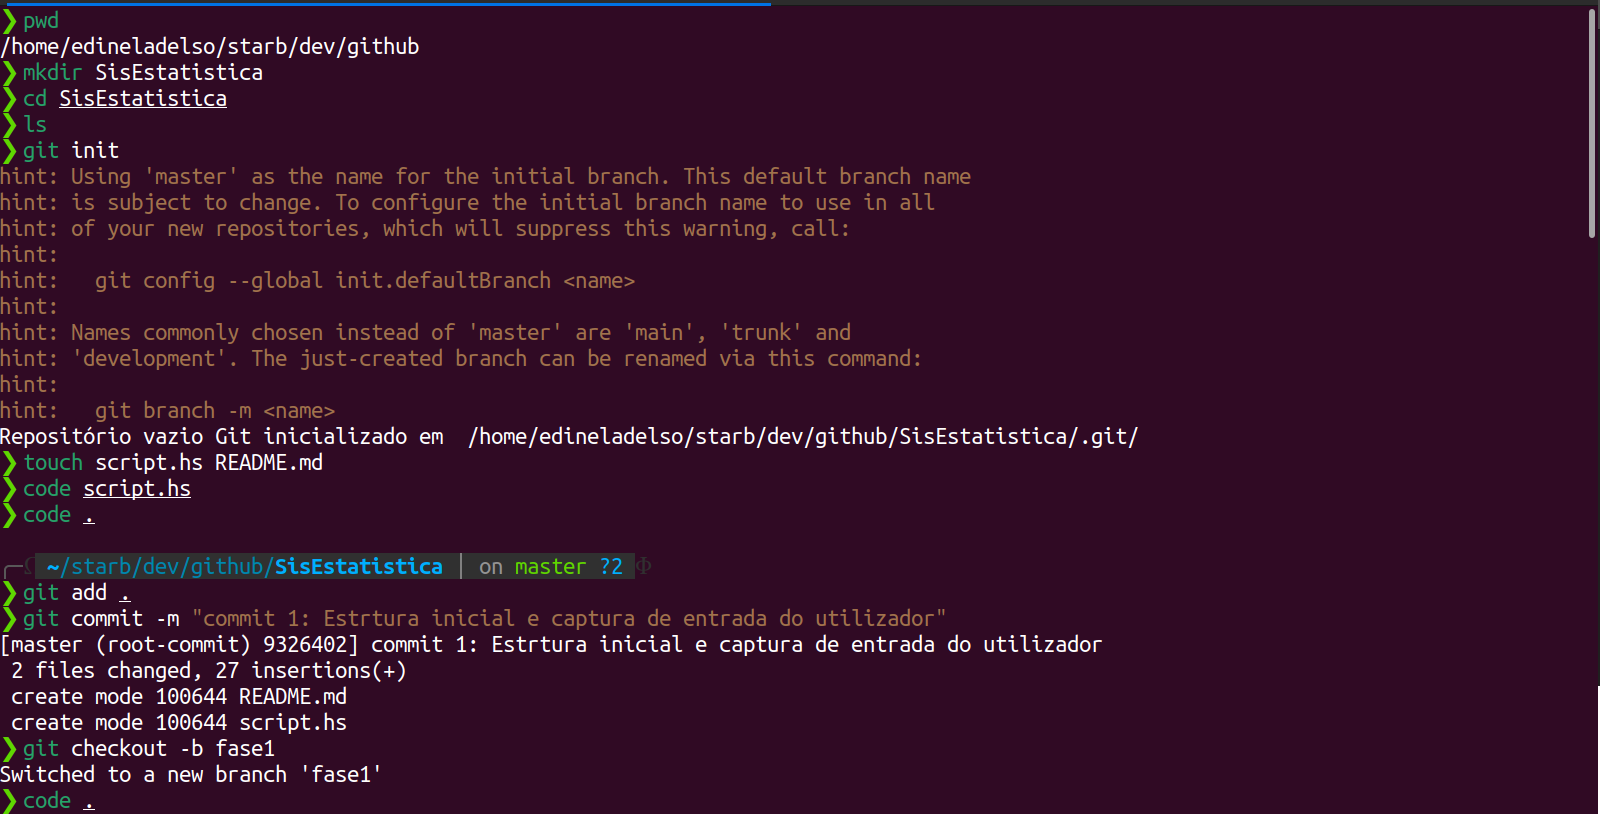
\includegraphics[width=\textwidth]{1000973638.png}
\caption{Criação do directório do projecto e inicialização do repositório Git.}
\label{fig:init}
\end{figure}

A figura~\ref{fig:init} mostra o terminal Linux após a execução dos comandos de inicialização. É possível observar: a confirmação do directório de trabalho pelo comando \texttt{pwd} (\texttt{/home/edineladelso/starb/dev/github}); a criação do directório \texttt{SisEstatistica}; a navegação para o interior do directório com \texttt{cd}; a execução de \texttt{git init} que inicializou o repositório vazio, tendo o Git emitido uma mensagem de aviso (\textit{hint}) a indicar que o nome da \textit{branch} inicial é \texttt{master} e que este comportamento pode ser reconfigurado; a criação dos ficheiros \texttt{script.hs} e \texttt{README.md} com o comando \texttt{touch}; e finalmente a execução dos comandos \texttt{git add .} e \texttt{git commit} que registaram o primeiro \textit{commit} do projecto com a mensagem \textit{"commit 1: Estrtura inicial e captura de entrada do utilizador"}, correspondendo à criação de 2 ficheiros com 27 inserções. Na parte inferior da figura é também visível a criação da \textit{branch} \texttt{fase1} com o comando \texttt{git checkout -b fase1} e a confirmação da mudança para a nova \textit{branch}.

\section{Implementação da Estrutura Inicial}

Na \textit{branch} \texttt{master}, foi implementada a estrutura base do programa em Haskell. Esta estrutura é responsável pela captura da entrada do utilizador, pela conversão da \textit{string} de entrada numa lista de números do tipo \texttt{Double} e pela validação básica da entrada.

O Código~\ref{lst:estrutura-inicial} apresenta o conteúdo do ficheiro \texttt{script.hs} após o primeiro \textit{commit}.

\begin{lstlisting}[style=haskell, caption={Estrutura inicial -- leitura e validação da entrada}, label=lst:estrutura-inicial]
-- Ficheiro: script.hs
-- Sistema de Estatistica de Listas em Haskell
-- Grupo 4

module Main where

-- Funcao principal que inicia a execucao do programa
main :: IO ()
main = do
    putStrLn "=================================="
    putStrLn "Sistema de Estatistica de listas"
    putStrLn "=================================="
    entrada <- getLine

    -- Converte a string de entrada numa lista de Double
    let listaNumeros = map read (words entrada) :: [Double]

    putStrLn "=========== RESULTADOS ==========="

    if null listaNumeros
        then putStrLn "Erro: A lista nao pode estar vazia!"
        else do
            putStrLn "\n--- Resultados ---"
            putStrLn ("Lista processada com sucesso: "
                        ++ show listaNumeros)
\end{lstlisting}

Analisando o código linha por linha: a declaração \texttt{module Main where} define o módulo principal do programa; a assinatura \texttt{main :: IO ()} especifica que a função \texttt{main} é uma acção de entrada/saída (\texttt{IO}) que não devolve valor; \texttt{putStrLn} imprime uma linha de texto no terminal; \texttt{getLine} lê uma linha de entrada do utilizador e armazena-a na variável \texttt{entrada}; a expressão \texttt{words entrada} divide a \textit{string} de entrada em palavras usando os espaços como separadores; \texttt{map read} aplica a função \texttt{read} a cada palavra, convertendo-a para o tipo \texttt{Double}; a anotação \texttt{:: [Double]} especifica explicitamente o tipo da lista resultante; \texttt{null listaNumeros} verifica se a lista está vazia; e o bloco \texttt{do} com indentação dentro do \texttt{else} executa as acções sequencialmente quando a lista contém elementos.

\section{Desenvolvimento da Branch \texttt{fase1}}

Após o primeiro \textit{commit} na \textit{branch} \texttt{master}, o desenvolvimento prosseguiu com a criação da \textit{branch} \texttt{fase1}, dedicada à implementação das funções de cálculo da soma e da média.

\subsection{Criação da Branch e Conceito de Ramificação}

O comando utilizado para criar e mudar simultaneamente para a nova \textit{branch} foi:

\begin{lstlisting}[style=bash, caption={Criação da branch fase1}, label=lst:checkout-fase1]
git checkout -b fase1
\end{lstlisting}

{\sloppy O parâmetro \texttt{-b} instrui o Git a criar uma nova \textit{branch} com o nome especificado (\texttt{fase1}) e a mudar imediatamente para ela. Uma \textit{branch} no Git é essencialmente um ponteiro leve para um \textit{commit} específico, que avança automaticamente a cada novo \textit{commit} realizado nessa \textit{branch}. A criação de uma \textit{branch} para cada fase de desenvolvimento garante que as alterações em curso não interferem com o código estável da \textit{branch} principal, permitindo trabalhar de forma isolada e segura.}

\subsection{Implementação de \texttt{calcularSoma} e \texttt{calcularMedia}}

Na \textit{branch} \texttt{fase1}, foram implementadas as funções \texttt{calcularSoma} e \mbox{\texttt{calcularMedia}}:

\begin{lstlisting}[style=haskell, caption={Funções calcularSoma e calcularMedia -- branch fase1}, label=lst:fase1]
-- Funcao que calcula a soma de todos os elementos
calcularSoma :: [Double] -> Double
calcularSoma [] = 0
calcularSoma xs = sum xs

-- Funcao que calcula a media aritmetica
calcularMedia :: [Double] -> Double
calcularMedia xs = calcularSoma xs / fromIntegral (length xs)
\end{lstlisting}

A função \texttt{calcularSoma} utiliza correspondência de padrões (\textit{pattern matching}): quando recebe uma lista vazia \texttt{[]}, devolve \texttt{0}; para qualquer outra lista \texttt{xs}, aplica a função nativa do Haskell \texttt{sum}, que calcula a soma de todos os elementos. A função \texttt{calcularMedia} divide a soma total (obtida por \texttt{calcularSoma xs}) pelo número de elementos da lista. A conversão \texttt{fromIntegral} é necessária porque \texttt{length} devolve um valor do tipo \texttt{Int}, enquanto a divisão requer ambos os operandos do tipo \texttt{Double}.

\begin{figure}[H]
\centering
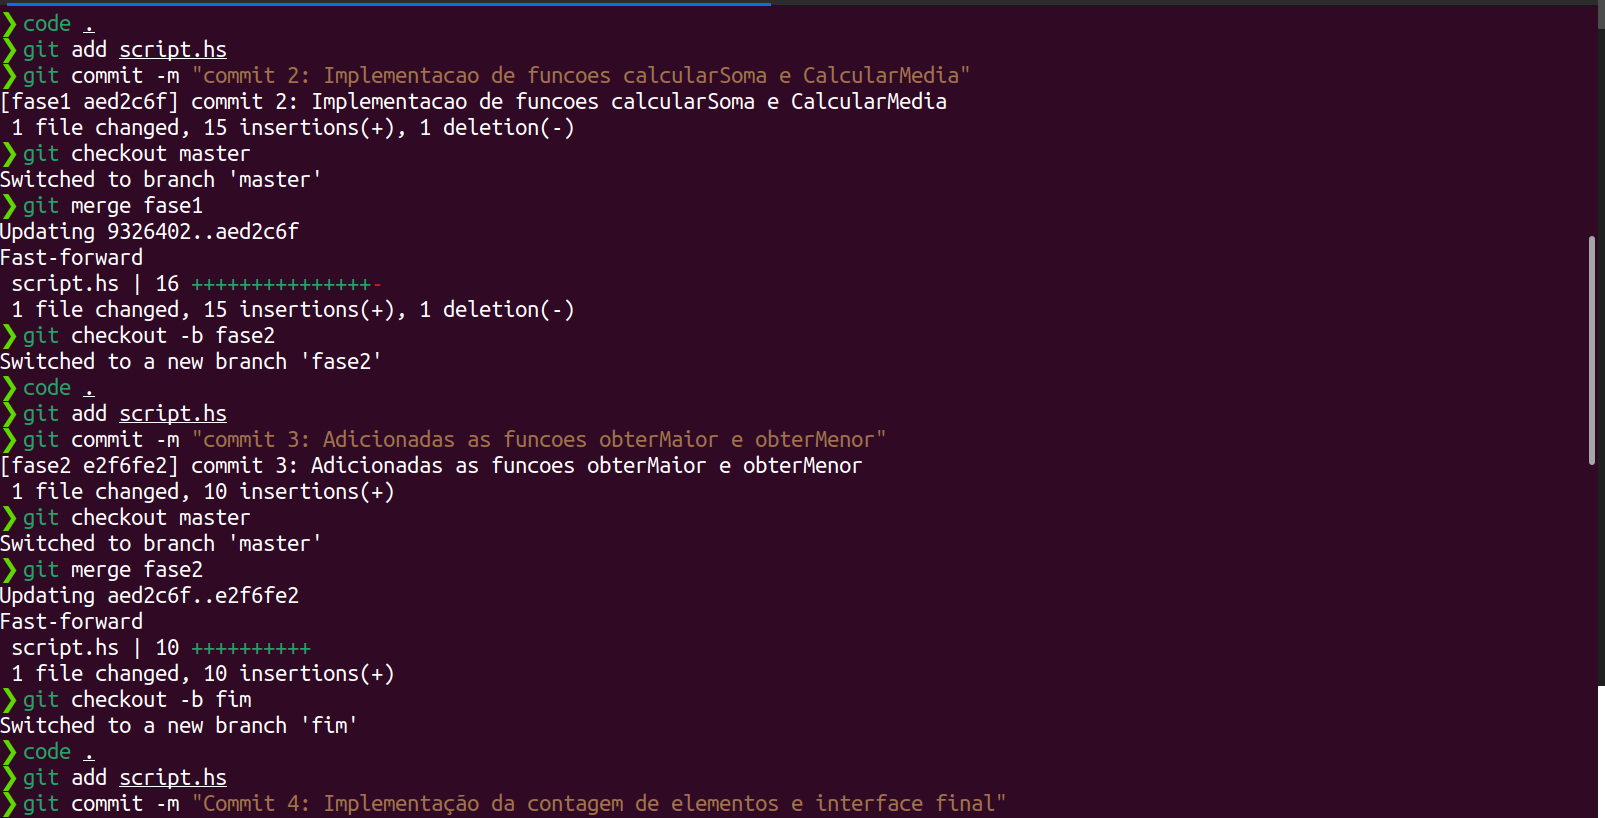
\includegraphics[width=\textwidth]{1000973639.png}
\caption{Criação da branch \texttt{fase1}, commits e merge para a branch \texttt{master}, seguidos da criação da branch \texttt{fase2}.}
\label{fig:fase1-fase2}
\end{figure}

A figura~\ref{fig:fase1-fase2} documenta o fluxo completo de desenvolvimento das \textit{branches} \texttt{fase1} e \texttt{fase2}. Na parte superior da imagem, observa-se o \textit{commit} 2 na \textit{branch} \texttt{fase1} com a mensagem \textit{"commit 2: Implementacao de funcoes calcularSoma e CalcularMedia"}, indicando que 1 ficheiro foi alterado com 15 inserções e 1 remoção. De seguida, o regresso à \textit{branch} \texttt{master} com \texttt{git checkout master} e a integração via \texttt{git merge fase1}, que produziu um \textit{merge} do tipo \textit{Fast-forward}, actualizando o ponteiro de \texttt{9326402} para \texttt{aed2c6f}.

\section{Integração da Branch \texttt{fase1} na Branch Principal}

Após a conclusão e teste das funções implementadas na \textit{branch} \texttt{fase1}, procedeu-se à sua integração na \textit{branch} \texttt{master}:

\begin{lstlisting}[style=bash, caption={Integração da branch fase1 na branch master}, label=lst:merge-fase1]
git checkout master
git merge fase1
\end{lstlisting}

O resultado do \textit{merge} foi do tipo \textit{Fast-forward}, o que significa que a \textit{branch} \texttt{master} não continha \textit{commits} novos desde a criação da \textit{branch} \texttt{fase1}. Neste caso, o Git simplesmente avança o ponteiro da \textit{branch} \texttt{master} para apontar para o \textit{commit} mais recente da \textit{branch} \texttt{fase1}, sem criar um \textit{commit} de \textit{merge} adicional.

A figura~\ref{fig:merge-tikz} ilustra graficamente o fluxo de desenvolvimento com \textit{branches} e \textit{merges} utilizado neste projeto.

\begin{figure}[H]
\centering
\begin{tikzpicture}[
  node distance=1.8cm and 2.2cm,
  commit/.style={circle, draw=MidnightBlue, fill=MidnightBlue!15, minimum size=0.9cm, font=\footnotesize\ttfamily},
  branch/.style={rectangle, rounded corners, draw=OliveGreen, fill=OliveGreen!10, minimum width=1.8cm, minimum height=0.6cm, font=\footnotesize\bfseries},
  arrow/.style={-{Stealth}, thick, MidnightBlue},
  merge/.style={-{Stealth}, thick, dashed, BrickRed},
]

% Commits master
\node[commit] (c1) {C1};
\node[commit, right=of c1] (c2m) {};
\node[commit, right=of c2m] (c3m) {};
\node[commit, right=of c3m] (c4m) {};
\node[commit, right=of c4m] (c5) {C5};

% Labels master
\node[branch, above=0.3cm of c1] {master};

% Branch fase1
\node[commit, above=1.5cm of c2m] (c2f1) {C2};
\node[branch, above=0.3cm of c2f1] {fase1};

% Branch fase2
\node[commit, above=1.5cm of c3m] (c3f2) {C3};
\node[branch, above=0.3cm of c3f2] {fase2};

% Branch fim
\node[commit, above=1.5cm of c4m] (c4fim) {C4};
\node[branch, above=0.3cm of c4fim] {fim};

% Arrows master
\draw[arrow] (c1) -- (c2m);
\draw[arrow] (c2m) -- (c3m);
\draw[arrow] (c3m) -- (c4m);
\draw[arrow] (c4m) -- (c5);

% Branch arrows
\draw[arrow] (c1) -- (c2f1);
\draw[arrow] (c2m.north) -- (c3f2);
\draw[arrow] (c3m.north) -- (c4fim);

% Merge arrows
\draw[merge] (c2f1) -- node[right, font=\tiny] {merge} (c2m);
\draw[merge] (c3f2) -- node[right, font=\tiny] {merge} (c3m);
\draw[merge] (c4fim) -- node[right, font=\tiny] {merge} (c4m);

% Labels commits master
\node[below=0.2cm of c1, font=\tiny] {init};
\node[below=0.2cm of c2m, font=\tiny] {ff fase1};
\node[below=0.2cm of c3m, font=\tiny] {ff fase2};
\node[below=0.2cm of c4m, font=\tiny] {ff fim};
\node[below=0.2cm of c5, font=\tiny] {README};

\end{tikzpicture}
\caption{Diagrama do fluxo de desenvolvimento com \textit{branches} e \textit{merges} (Fast-forward).}
\label{fig:merge-tikz}
\end{figure}

\section{Desenvolvimento da Branch \texttt{fase2}}

Com a \textit{branch} \texttt{fase1} integrada com sucesso na \textit{branch} \texttt{master}, prosseguiu-se com a criação da \textit{branch} \texttt{fase2} para implementação das funções de determinação do maior e do menor valor.

\begin{lstlisting}[style=bash, caption={Criação da branch fase2}, label=lst:checkout-fase2]
git checkout -b fase2
\end{lstlisting}

Conforme visível na figura~\ref{fig:fase1-fase2}, o Git confirmou a criação e mudança para a nova \textit{branch} com a mensagem \textit{"Switched to a new branch 'fase2'"}.

\subsection{Implementação das Funções obterMaior e obterMenor}

As funções \texttt{obterMaior} e \texttt{obterMenor} foram implementadas recorrendo às funções nativas do Prelude do Haskell:

\begin{lstlisting}[style=haskell, caption={Funções obterMaior e obterMenor -- branch fase2}, label=lst:fase2]
-- Funcao para encontrar o maior valor da lista
obterMaior :: [Double] -> Double
obterMaior xs = maximum xs

-- Funcao para encontrar o menor valor da lista
obterMenor :: [Double] -> Double
obterMenor xs = minimum xs
\end{lstlisting}

A função \texttt{maximum} percorre a lista e devolve o elemento de maior valor, utilizando a relação de ordem definida para o tipo \texttt{Double}. De forma análoga, \texttt{minimum} devolve o elemento de menor valor. Ambas as funções são polimórficas e operam sobre qualquer tipo que implemente a classe de tipos \texttt{Ord} (tipos ordenáveis).

O \textit{commit} 3 na \textit{branch} \texttt{fase2} foi registado com a mensagem \textit{"commit 3: Adicionadas as funcoes obterMaior e obterMenor"}, com 1 ficheiro modificado e 10 inserções, conforme visível na figura~\ref{fig:fase1-fase2}. A integração na \textit{branch} \texttt{master} foi realizada via \texttt{git merge fase2}, resultando novamente num \textit{merge} do tipo \textit{Fast-forward}, actualizando o ponteiro de \texttt{aed2c6f} para \texttt{e2f6fe2}.

\section{Integração da Branch \texttt{fase2}}

\begin{lstlisting}[style=bash, caption={Integração da branch fase2 na branch master}, label=lst:merge-fase2]
git checkout master
git merge fase2
\end{lstlisting}

\section{Desenvolvimento da Branch \texttt{fim}}

A fase final do desenvolvimento correspondeu à criação da \textit{branch} \texttt{fim}, na qual foi implementada a função de contagem de elementos e finalizada a interface do programa.

\begin{lstlisting}[style=bash, caption={Criação da branch fim}, label=lst:checkout-fim]
git checkout -b fim
\end{lstlisting}

\begin{lstlisting}[style=haskell, caption={Função contarElementos -- branch fim}, label=lst:contarElementos]
-- Funcao para contar a quantidade de elementos
contarElementos :: [Double] -> Int
contarElementos xs = length xs
\end{lstlisting}

A função \texttt{length} do Prelude do Haskell devolve o número de elementos de uma lista como um valor do tipo \texttt{Int}. A sua utilização é directa e eficiente para a maioria dos casos práticos.

\begin{figure}[H]
\centering
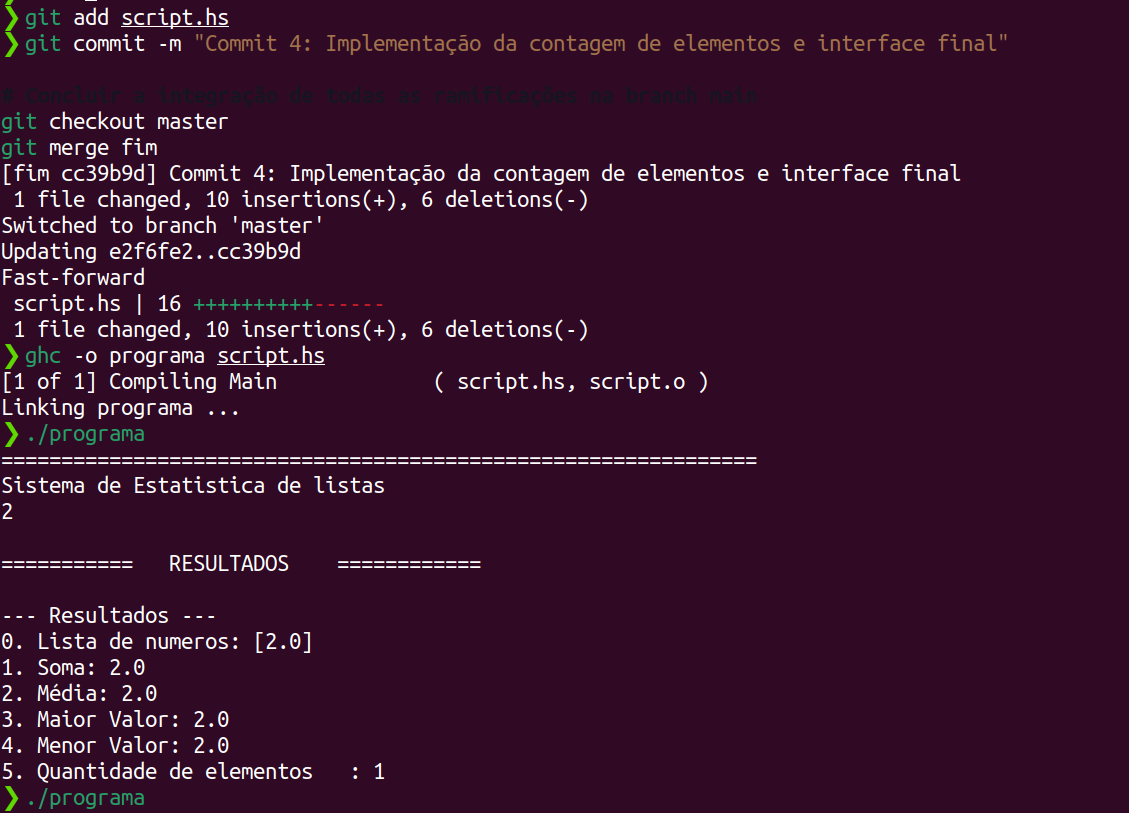
\includegraphics[width=\textwidth]{1000973643.png}
\caption{Implementação da fase final: commit 4, integração da branch \texttt{fim} na \texttt{master} e primeira execução do programa compilado.}
\label{fig:fim}
\end{figure}

A figura~\ref{fig:fim} documenta a fase final do desenvolvimento. Observam-se os seguintes passos: o \textit{commit} 4 com a mensagem \textit{"Commit 4: Implementação da contagem de elementos e interface final"}; o regresso à \textit{branch} \texttt{master} com \texttt{git checkout master}; o \textit{merge} da \textit{branch} \texttt{fim} (\texttt{git merge fim}), que produziu novamente um \textit{Fast-forward} de \texttt{e2f6fe2} para \texttt{cc39b9d}; a compilação do programa com o comando \texttt{ghc -o programa script.hs}, que produziu o executável \texttt{programa} a partir do módulo \texttt{Main} em \texttt{script.hs}; e a primeira execução do programa compilado com \texttt{./programa}, introduzindo o valor \texttt{2} e verificando que os resultados (Soma: 2.0, Média: 2.0, Maior Valor: 2.0, Menor Valor: 2.0, Quantidade: 1) são correctos.

\section{Código Final Completo}

O código final completo do Sistema de Estatística de Listas, resultante da integração de todas as \textit{branches}, é apresentado no Código~\ref{lst:codigo-final}.

\begin{lstlisting}[style=haskell, caption={Código final completo do Sistema de Estatística de Listas}, label=lst:codigo-final]
-- Ficheiro: script.hs
-- Sistema de Estatistica de Listas em Haskell
-- Grupo 4 -- Licenciatura em Informatica

module Main where

-- Funcao que calcula a soma de todos os elementos
calcularSoma :: [Double] -> Double
calcularSoma [] = 0
calcularSoma xs = sum xs

-- Funcao que calcula a media aritmetica
calcularMedia :: [Double] -> Double
calcularMedia xs = calcularSoma xs / fromIntegral (length xs)

-- Funcao para encontrar o maior valor da lista
obterMaior :: [Double] -> Double
obterMaior xs = maximum xs

-- Funcao para encontrar o menor valor da lista
obterMenor :: [Double] -> Double
obterMenor xs = minimum xs

-- Funcao para contar a quantidade de elementos
contarElementos :: [Double] -> Int
contarElementos xs = length xs

-- Funcao principal do programa
main :: IO ()
main = do
    putStrLn "=================================="
    putStrLn "Sistema de Estatistica de listas"
    putStrLn "=================================="
    entrada <- getLine

    let listaNumeros = map read (words entrada) :: [Double]

    putStrLn "=========== RESULTADOS ==========="

    if null listaNumeros
        then putStrLn "Erro: A lista nao pode estar vazia!"
        else do
            putStrLn "\n--- Resultados ---"
            putStrLn ("0. Lista de numeros: "
                        ++ show listaNumeros)
            putStrLn ("1. Soma: "
                        ++ show (calcularSoma listaNumeros))
            putStrLn ("2. Media: "
                        ++ show (calcularMedia listaNumeros))
            putStrLn ("3. Maior Valor: "
                        ++ show (obterMaior listaNumeros))
            putStrLn ("4. Menor Valor: "
                        ++ show (obterMenor listaNumeros))
            putStrLn ("5. Quantidade de elementos   : "
                        ++ show (contarElementos listaNumeros))
\end{lstlisting}

% ============================================================
%  CAPÍTULO 4 — TESTES E RESULTADOS
% ============================================================
\chapter{Testes e Resultados}

A fase de testes constitui uma etapa fundamental do processo de desenvolvimento de software, permitindo validar a correção dos algoritmos implementados e identificar comportamentos inesperados. Neste capítulo são apresentados e analisados os resultados dos testes realizados com diferentes entradas.

\section{Compilação do Programa}

Antes da realização dos testes, o código Haskell foi compilado utilizando o GHC (\textit{Glasgow Haskell Compiler}):

\begin{lstlisting}[style=bash, caption={Compilação do programa com GHC}, label=lst:compilacao]
ghc -o programa script.hs
\end{lstlisting}

O GHC compilou o módulo \texttt{Main} do ficheiro \texttt{script.hs}, gerou o ficheiro objecto \texttt{script.o} e ligou (\textit{linked}) os módulos para produzir o executável \texttt{programa}. A compilação foi concluída sem erros, confirmando a correção sintáctica e semântica do código.

\section{Teste 1: Lista com Um Único Elemento}

\subsection{Entrada}

O primeiro teste foi realizado com uma lista contendo apenas um elemento: o valor \texttt{2}.

\begin{figure}[H]
\centering
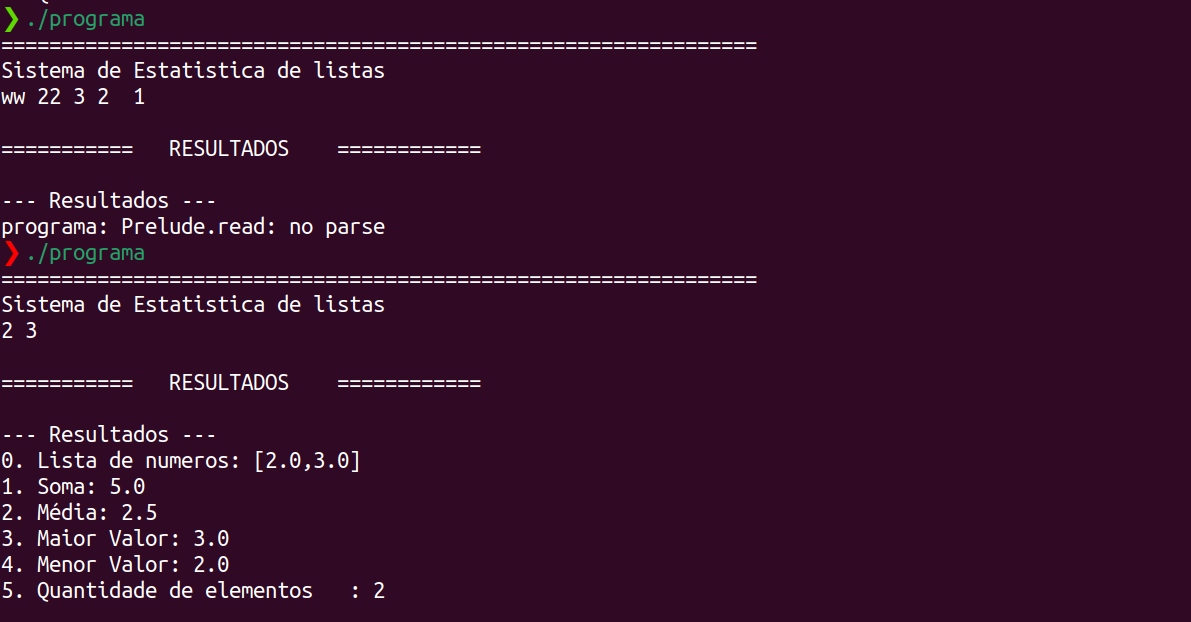
\includegraphics[width=\textwidth]{1000973642.png}
\caption{Execução do programa utilizando uma lista contendo um único elemento (valor 2).}
\label{fig:teste1}
\end{figure}

\subsection{Análise dos Resultados}

A figura~\ref{fig:teste1} apresenta a saída do programa para a entrada \texttt{2}. Os resultados obtidos foram:

\begin{table}[H]
\centering
\caption{Resultados do Teste 1 -- entrada: \{2\}}
\label{tab:teste1}
\begin{tabular}{lll}
\toprule
Métrica & Resultado Obtido & Verificação Matemática \\
\midrule
Lista & [2.0] & \{2\} \\
Soma & 2.0 & $\sum = 2$ \\
Média & 2.0 & $\bar{x} = 2/1 = 2$ \\
Maior Valor & 2.0 & $\max\{2\} = 2$ \\
Menor Valor & 2.0 & $\min\{2\} = 2$ \\
Quantidade & 1 & $|\{2\}| = 1$ \\
\bottomrule
\end{tabular}
\end{table}

Todos os resultados são matematicamente correctos. Para uma lista com um único elemento, é esperado que a soma, a média, o maior valor e o menor valor sejam todos iguais ao único elemento da lista. A quantidade é correctamente reportada como 1.

\section{Teste 2: Lista com Dois Elementos}

\subsection{Entrada}

O segundo teste utilizou a lista com dois elementos: \texttt{2 3}.

\begin{figure}[H]
\centering
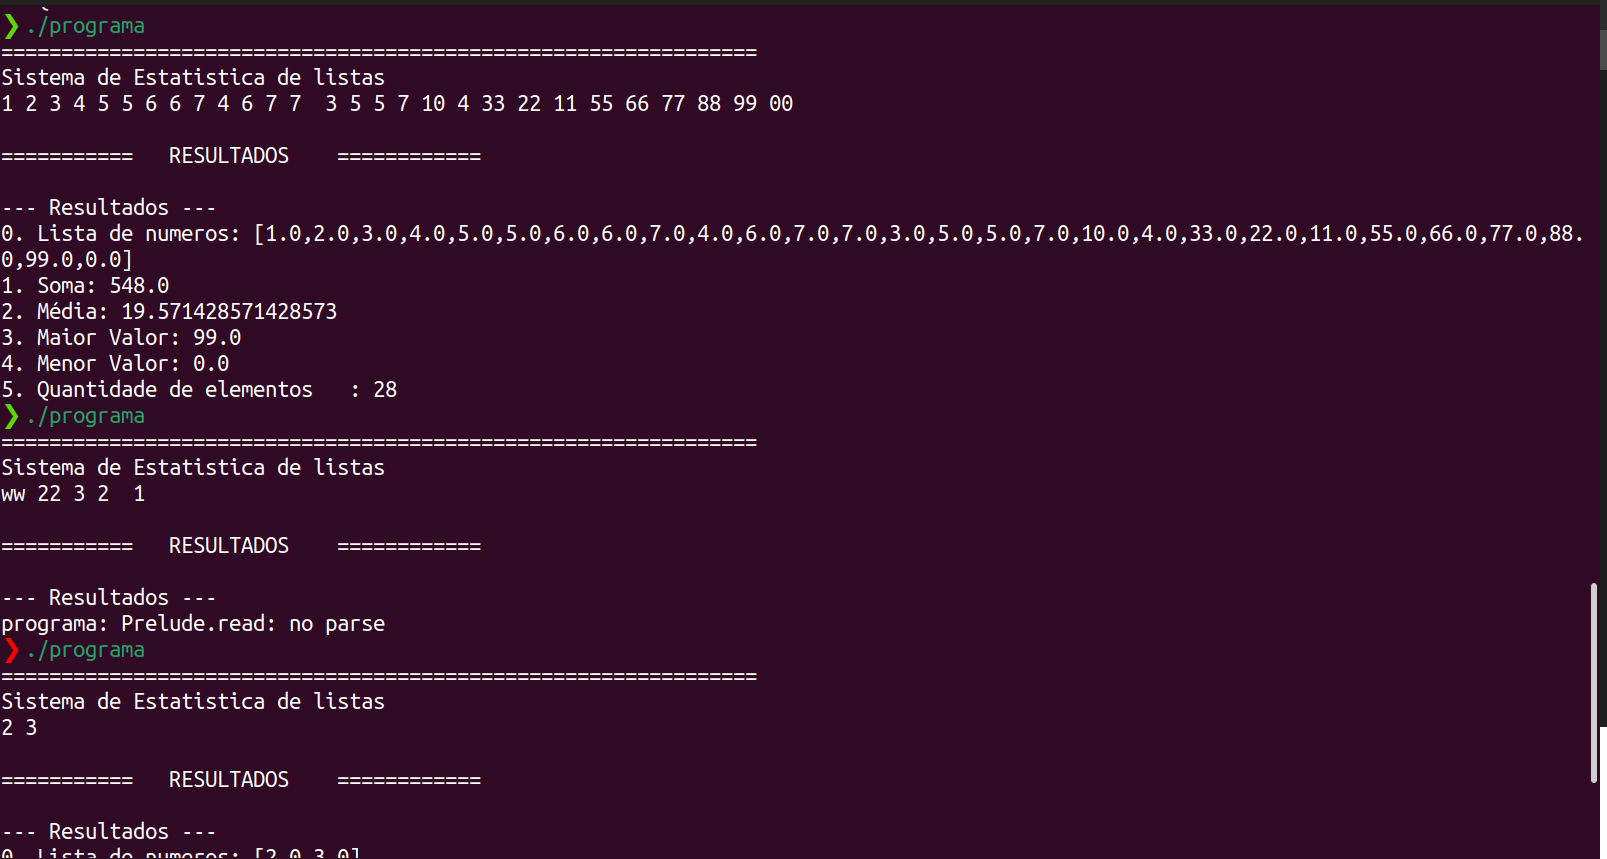
\includegraphics[width=0.95\textwidth]{1000973641.png}
\caption{Execução do sistema utilizando uma lista com dois elementos (2 e 3).}
\label{fig:teste2}
\end{figure}

\subsection{Análise dos Resultados}

A figura~\ref{fig:teste2} apresenta os resultados para a entrada \texttt{2 3}. A tabela~\ref{tab:teste2} valida matematicamente cada resultado obtido.

\begin{table}[H]
\centering
\caption{Resultados do Teste 2 -- entrada: \{2, 3\}}
\label{tab:teste2}
\begin{tabular}{lll}
\toprule
Métrica & Resultado Obtido & Verificação Matemática \\
\midrule
Lista & [2.0, 3.0] & \{2, 3\} \\
Soma & 5.0 & $2 + 3 = 5$ \\
Média & 2.5 & $5 / 2 = 2.5$ \\
Maior Valor & 3.0 & $\max\{2,3\} = 3$ \\
Menor Valor & 2.0 & $\min\{2,3\} = 2$ \\
Quantidade & 2 & $|\{2,3\}| = 2$ \\
\bottomrule
\end{tabular}
\end{table}

Todos os resultados estão matematicamente correctos. O teste valida o funcionamento correcto das cinco funções implementadas para uma lista com dois elementos distintos.

\section{Teste 3: Lista Extensa}

\subsection{Entrada}

O terceiro teste foi realizado com uma lista extensa de 28 elementos:

\begin{center}
\texttt{1 2 3 4 5 5 6 6 7 4 6 7 7 3 5 5 7 10 4 33 22 11 55 66 77 88 99 00}
\end{center}

\begin{figure}[H]
\centering
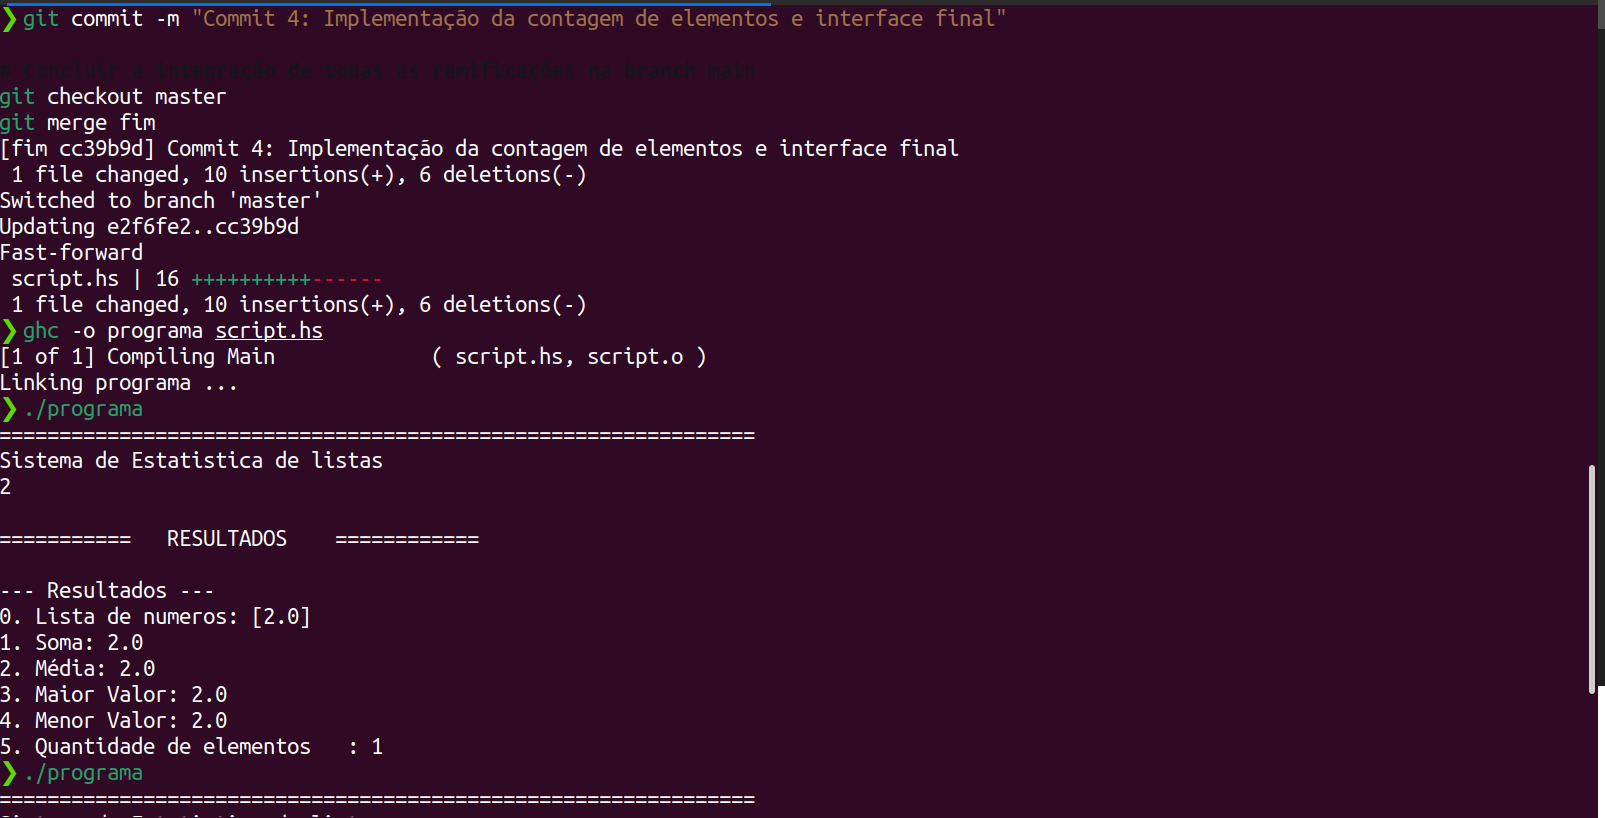
\includegraphics[width=\textwidth]{1000973640.png}
\caption{Execução do sistema utilizando uma lista extensa de 28 elementos para validação robusta do algoritmo.}
\label{fig:teste3}
\end{figure}

\subsection{Análise Matemática Completa}

\begin{table}[H]
\centering
\caption{Análise matemática completa -- Teste 3}
\label{tab:teste3}
\begin{tabular}{lll}
\toprule
Métrica & Resultado do Sistema & Verificação Matemática \\
\midrule
Quantidade & 28 & 28 elementos contados \\
Soma & 548.0 & Soma de todos os 28 elementos $= 548$ \\
Média & 19.571... & $548 \div 28 \approx 19{,}5714$ \\
Maior Valor & 99.0 & O maior elemento da lista é 99 \\
Menor Valor & 0.0 & O valor 00 é interpretado como 0 \\
\bottomrule
\end{tabular}
\end{table}

A média calculada pelo sistema, $19.571428571428573$, corresponde com precisão ao valor matemático exacto $548/28 = 19.\overline{571428}$. O valor \texttt{00} introduzido pelo utilizador é correctamente interpretado pelo Haskell como o número $0$, sendo reportado como o menor valor da lista.

\section{Teste de Entrada Inválida}

\subsection{Entrada}

O quarto teste foi realizado com uma entrada contendo uma sequência de caracteres inválida: \texttt{ww 22 3 2 1}, onde \texttt{ww} não pode ser convertido para um número do tipo \texttt{Double}.

\subsection{Comportamento do Sistema e Análise Técnica}

O sistema reportou o erro: \texttt{programa: Prelude.read: no parse}. Este comportamento é resultado do funcionamento da função \texttt{read} do Prelude do Haskell, que tenta converter uma \textit{string} para um tipo especificado. Quando a conversão não é possível (como é o caso de \texttt{"ww"} para o tipo \texttt{Double}), a função \texttt{read} lança uma excepção em tempo de execução com a mensagem \texttt{Prelude.read: no parse}.

A expressão \texttt{map read (words entrada) :: [Double]} processa a lista de palavras de forma sequential. Ao tentar converter \texttt{"ww"} para \texttt{Double}, a função \texttt{read} falha imediatamente e a excepção interrompe a execução do programa antes de qualquer cálculo ser efectuado.

Este comportamento, embora não tratado de forma elegante nesta versão do programa, é tecnicamente previsível e documentado. Uma versão mais robusta do sistema poderia utilizar a função \texttt{readMaybe} do módulo \texttt{Text.Read} para tratar este caso de forma segura, devolvendo um valor \texttt{Nothing} para entradas inválidas em vez de lançar uma excepção.

% ============================================================
%  CAPÍTULO 5 — ANÁLISE DO VERSIONAMENTO
% ============================================================
\chapter{Análise do Versionamento}

\section{Estrutura de Branches}

A tabela~\ref{tab:branches} apresenta a estrutura completa de \textit{branches} utilizada no projecto e o resultado de cada fase de desenvolvimento.

\begin{table}[H]
\centering
\caption{Análise das branches do projecto}
\label{tab:branches}
\begin{tabular}{p{2.5cm} p{5cm} p{5.5cm}}
\toprule
\bfseries Branch & \bfseries Objetivo & \bfseries Resultado \\
\midrule
\texttt{master} & Ramo principal. Estrutura base e captura de entrada do utilizador. & Ficheiros iniciais criados (\texttt{script.hs}, \texttt{README.md}). Primeiro \textit{commit} registado com o hash \texttt{9326402}. \\
\addlinespace
\texttt{fase1} & Implementação das funções de cálculo da soma e da média aritmética. & Funções \texttt{calcularSoma} e \texttt{calcularMedia} implementadas e testadas. Commit \texttt{aed2c6f}. Integrada na \texttt{master} via \textit{fast-forward}. \\
\addlinespace
\texttt{fase2} & Implementação das funções de determinação do maior e do menor valor da lista. & Funções \texttt{obterMaior} e \texttt{obterMenor} implementadas. Commit \texttt{e2f6fe2}. Integrada na \texttt{master} via \textit{fast-forward}. \\
\addlinespace
\texttt{fim} & Implementação da função de contagem de elementos e finalização da interface do programa. & Função \texttt{contarElementos} implementada. Interface final definida. Commit \texttt{cc39b9d}. Integrada na \texttt{master} via \textit{fast-forward}. \\
\bottomrule
\end{tabular}
\end{table}

\section{Linha Temporal dos Commits}

A tabela~\ref{tab:commits} apresenta a cronologia completa dos \textit{commits} realizados ao longo do desenvolvimento do projecto.

\begin{table}[H]
\centering
\caption{Linha temporal dos commits do projecto}
\label{tab:commits}
\begin{tabular}{p{1.2cm} p{2.2cm} p{8.8cm}}
\toprule
\bfseries \# & \bfseries Branch & \bfseries Descrição do Commit \\
\midrule
1 & \texttt{master} & Estrutura inicial e captura de entrada do utilizador. Criação dos ficheiros \texttt{script.hs} e \texttt{README.md} com a estrutura base do programa e a lógica de leitura e conversão da entrada. \\
\addlinespace
2 & \texttt{fase1} & Implementação das funções \texttt{calcularSoma} e \texttt{calcularMedia}. Adição das duas primeiras métricas estatísticas e actualização da função \texttt{main} para exibir os resultados. \\
\addlinespace
3 & \texttt{fase2} & Adição das funções \texttt{obterMaior} e \texttt{obterMenor}. Extensão do sistema com as funções de determinação dos valores extremos da lista. \\
\addlinespace
4 & \texttt{fim} & Implementação da contagem de elementos e interface final. Adição da função \texttt{contarElementos} e refinamento da interface de saída do programa. \\
\addlinespace
5 & \texttt{master} & Actualização completa do ficheiro \texttt{README.md} com documentação do projecto, instruções de compilação e execução, e descrição das funcionalidades. \\
\bottomrule
\end{tabular}
\end{table}

% ============================================================
%  CAPÍTULO 6 — DIFICULDADES ENCONTRADAS
% ============================================================
\chapter{Dificuldades Encontradas}

\section{Conversão de Strings para Double}

Uma das principais dificuldades encontradas durante o desenvolvimento foi a correcta conversão dos dados de entrada, fornecidos pelo utilizador como uma \textit{string}, para valores numéricos do tipo \texttt{Double}. Em Haskell, esta conversão exige a combinação das funções \texttt{words} (para separar a \textit{string} em palavras), \texttt{map} (para aplicar uma função a cada elemento da lista) e \texttt{read} (para converter cada palavra para o tipo desejado), bem como a anotação de tipo explícita \texttt{:: [Double]} para informar o compilador do tipo pretendido.

A necessidade da conversão \texttt{fromIntegral} na função \texttt{calcularMedia}, para compatibilizar o resultado inteiro de \texttt{length} com o tipo \texttt{Double} da divisão, foi igualmente uma fonte de confusão inicial, ilustrando a rigidez do sistema de tipos de Haskell.

\section{Tratamento de Listas Vazias}

O tratamento de listas vazias constituiu outro desafio técnico relevante. As funções \texttt{maximum} e \texttt{minimum} do Prelude do Haskell lançam uma excepção quando aplicadas a uma lista vazia. Por isso, foi necessário implementar uma verificação prévia com a função \texttt{null} na função \texttt{main}, de forma a garantir que as funções de cálculo não são invocadas com uma lista vazia.

\section{Utilização de Branches no Git}

A adopção de um modelo de desenvolvimento baseado em \textit{branches} exigiu uma compreensão clara dos conceitos de criação de \textit{branches}, mudança entre \textit{branches} e integração via \textit{merge}. A principal dificuldade residiu em compreender a diferença entre um \textit{merge} do tipo \textit{fast-forward} e um \textit{merge} com criação de \textit{commit} adicional, bem como as situações em que cada tipo de \textit{merge} ocorre.

\section{Integração via Merge}

A sequência correcta de comandos para integrar uma \textit{branch} na \textit{branch} principal exige que o utilizador regresse primeiro à \textit{branch} de destino (\texttt{git checkout master}) antes de executar o \textit{merge} (\texttt{git merge nome-da-branch}). A realização do \textit{merge} na \textit{branch} errada poderia ter consequências negativas para o histórico do projecto.

\section{Testes e Validação}

A definição de casos de teste representativos, incluindo casos extremos como listas com um único elemento e entradas inválidas, exigiu um esforço de análise e criatividade por parte do grupo. O comportamento do sistema perante entradas inválidas, manifestado pela excepção \texttt{Prelude.read: no parse}, revelou a importância de implementar tratamento robusto de erros em aplicações de produção.

% ============================================================
%  CAPÍTULO 7 — CONCLUSÕES
% ============================================================
\chapter{Conclusões}

\section{Síntese do Trabalho Realizado}

O presente trabalho teve como objectivo o desenvolvimento de um Sistema de Estatística de Listas em Haskell, utilizando o ambiente Linux, o sistema de controlo de versões Git e a plataforma GitHub para hospedagem remota do código. O sistema foi desenvolvido com sucesso, implementando todas as funcionalidades propostas: cálculo da soma, da média, do maior valor, do menor valor e da quantidade de elementos de uma lista numérica fornecida pelo utilizador.

O desenvolvimento seguiu uma metodologia de desenvolvimento incremental baseada em \textit{branches}, com quatro fases claramente delimitadas e documentadas. Cada fase foi registada num \textit{commit} Git com mensagem descritiva, produzindo um histórico de versões limpo e rastreável. As integrações entre \textit{branches} foram realizadas com sucesso através de operações de \textit{merge} do tipo \textit{fast-forward}, o que reflecte a organização sequencial e não divergente do processo de desenvolvimento adoptado.

\section{Objectivos Atingidos}

Todos os objectivos específicos definidos na secção de introdução foram alcançados. A função \texttt{calcularSoma} calcula correctamente a soma de todos os elementos da lista. A função \texttt{calcularMedia} determina a média aritmética com precisão de ponto flutuante. As funções \texttt{obterMaior} e \texttt{obterMenor} identificam correctamente os valores extremos da lista. A função \texttt{contarElementos} reporta com precisão o número de elementos. Os três testes principais com listas de dimensões variadas (1, 2 e 28 elementos) confirmaram a correção dos algoritmos em todos os casos.

A utilização do Git e do GitHub foi demonstrada através de um histórico de 5 \textit{commits} distribuídos por 4 \textit{branches}, documentando rigorosamente o processo de desenvolvimento incremental. O README.md foi actualizado com instruções completas de utilização do projecto.

\section{Aprendizagem de Haskell}

O desenvolvimento deste projecto proporcionou ao Grupo 4 uma primeira experiência prática significativa com a linguagem Haskell e o paradigma de programação funcional. A compreensão dos conceitos de correspondência de padrões (\textit{pattern matching}), tipagem estática forte, funções de ordem superior (\texttt{map}), e a distinção entre tipos \texttt{Int} e \texttt{Double} foi aprofundada através da prática efectiva.

A experiência revelou que Haskell, apesar de exigir uma curva de aprendizagem mais íngreme do que as linguagens imperativas convencionais, oferece uma forma de expressão de algoritmos que é simultaneamente concisa e matematicamente rigorosa. O código produzido é compacto, legível e directamente mapeável para as definições matemáticas das operações estatísticas implementadas.

\section{Aprendizagem de Git e GitHub}

A utilização prática do Git ao longo deste projecto consolidou a compreensão de um conjunto essencial de operações de controlo de versões: \texttt{git init}, \texttt{git add}, \texttt{git commit}, \texttt{git checkout -b}, \texttt{git merge}. A observação directa dos hashes de \textit{commit} e das mensagens de \textit{fast-forward} no terminal permitiu compreender o funcionamento interno do sistema de referências do Git de uma forma que a leitura teórica não poderia proporcionar.

O GitHub, como plataforma de hospedagem remota, demonstrou a sua utilidade para a partilha e preservação do código. A atualização do README.md com documentação do projecto é uma prática profissional de valor elevado, que facilita a compreensão do projecto por parte de terceiros e serve como referência rápida para os próprios membros da equipa.

\section{Importância do Versionamento}

Este projecto demonstrou de forma concreta a importância do controlo de versões no desenvolvimento de software. A capacidade de registar o histórico completo das alterações, de trabalhar em funcionalidades isoladas sem risco de comprometer o código estável, e de integrar contribuições de forma organizada são vantagens que se manifestam mesmo em projectos de pequena dimensão como este. Em projectos de maior envergadura, com múltiplos colaboradores e funcionalidades complexas, estas vantagens tornam-se absolutamente indispensáveis.

O modelo de \textit{branches} adoptado neste projecto, apesar de simplificado relativamente aos modelos profissionais como o Git Flow ou o GitHub Flow, ilustra os princípios fundamentais do desenvolvimento paralelo e da integração contínua.

\section{Importância do Linux}

O ambiente Linux revelou-se o contexto ideal para o desenvolvimento deste projecto. A disponibilidade nativa do GHC (\textit{Glasgow Haskell Compiler}), a integração directa entre o terminal e as ferramentas de desenvolvimento, e a ausência de fricção no fluxo de trabalho entre o editor de código, o compilador, o Git e o terminal contribuíram para uma experiência de desenvolvimento fluída e eficiente.

O domínio dos comandos fundamentais do terminal Linux (\texttt{pwd}, \texttt{mkdir}, \texttt{cd}, \texttt{ls}, \texttt{touch}) é uma competência transversal de elevado valor para qualquer profissional de informatica onde o Linux é omnipresente.

\section{Considerações Finais}

O Sistema de Estatística de Listas desenvolvido constitui um exemplo bem-sucedido de aplicação integrada de múltiplas competências técnicas: programação funcional em Haskell, utilização profissional do terminal Linux e adopção de boas práticas de controlo de versões com Git e GitHub. O Grupo 4 considera que os objectivos académicos e técnicos do projecto foram plenamente alcançados, e que as competências adquiridas serão de utilidade directa em contextos profissionais futuros.

% ============================================================
%  REFERÊNCIAS BIBLIOGRÁFICAS
% ============================================================
\chapter*{Referências Bibliográficas}
\addcontentsline{toc}{chapter}{Referências Bibliográficas}

\begin{enumerate}[label={[{{\arabic*}}]}]

\item B. O'Sullivan, J. Goerzen, and D. Stewart, \textit{Real World Haskell}. Sebastopol, CA, USA: O'Reilly Media, 2009.

\item G. Hutton, \textit{Programming in Haskell}, 2nd ed. Cambridge, UK: Cambridge University Press, 2016.

\item The GHC Team, \textit{The Glorious Glasgow Haskell Compilation System User's Guide}, Version 9.x. Glasgow, UK: University of Glasgow, 2024. [Online]. Available: \url{https://downloads.haskell.org/ghc/latest/docs/users_guide/}

\item S. Chacon and B. Straub, \textit{Pro Git}, 2nd ed. Apress, 2014. [Online]. Available: \url{https://git-scm.com/book/en/v2}

\item Linux Foundation, \textit{Introduction to Linux}. San Francisco, CA, USA: The Linux Foundation, 2023. [Online]. Available: \url{https://www.linuxfoundation.org/}

\item GitHub, Inc., \textit{GitHub Documentation}. San Francisco, CA, USA: GitHub, Inc., 2024. [Online]. Available: \url{https://docs.github.com/}

\item P. Hudak, J. Hughes, S. Peyton Jones, and P. Wadler, ``A History of Haskell: Being Lazy with Class,'' in \textit{Proc. 3rd ACM SIGPLAN Conf. on History of Programming Languages (HOPL-III)}, San Diego, CA, USA, Jun. 2007, pp. 12-1--12-55.

\item W. Shotts, \textit{The Linux Command Line}, 5th ed. San Francisco, CA, USA: No Starch Press, 2019.

\item H. Lipovaca, \textit{Learn You a Haskell for Great Good!: A Beginner's Guide}. San Francisco, CA, USA: No Starch Press, 2011.

\item R. Leshchinskiy and contributors, \textit{Haskell 2010 Language Report}. Haskell.org, 2010. [Online]. Available: \url{https://www.haskell.org/onlinereport/haskell2010/}

\end{enumerate}

\clearpage

% ============================================================
%  APÊNDICE A — CÓDIGO-FONTE COMPLETO
% ============================================================
\appendix
\chapter{Código-Fonte Completo}

O código-fonte completo do Sistema de Estatística de Listas, conforme implementado e submetido ao repositório GitHub do Grupo 4, é apresentado a seguir.

\begin{lstlisting}[style=haskell, caption={Código-fonte completo -- script.hs}, label=lst:apendice-codigo]
-- Ficheiro: script.hs
-- Sistema de Estatistica de Listas em Haskell
-- Grupo 4 -- Licenciatura em Informatica

module Main where

-- Calcula a soma de todos os elementos da lista
calcularSoma :: [Double] -> Double
calcularSoma [] = 0
calcularSoma xs = sum xs

-- Calcula a media aritmetica da lista
calcularMedia :: [Double] -> Double
calcularMedia xs = calcularSoma xs / fromIntegral (length xs)

-- Devolve o maior valor da lista
obterMaior :: [Double] -> Double
obterMaior xs = maximum xs

-- Devolve o menor valor da lista
obterMenor :: [Double] -> Double
obterMenor xs = minimum xs

-- Devolve a quantidade de elementos da lista
contarElementos :: [Double] -> Int
contarElementos xs = length xs

-- Funcao principal
main :: IO ()
main = do
    putStrLn "=================================="
    putStrLn "Sistema de Estatistica de listas"
    putStrLn "=================================="
    entrada <- getLine
    let listaNumeros = map read (words entrada) :: [Double]
    putStrLn "=========== RESULTADOS ==========="
    if null listaNumeros
        then putStrLn "Erro: A lista nao pode estar vazia!"
        else do
            putStrLn "\n--- Resultados ---"
            putStrLn ("0. Lista de numeros: "
                        ++ show listaNumeros)
            putStrLn ("1. Soma: "
                        ++ show (calcularSoma listaNumeros))
            putStrLn ("2. Media: "
                        ++ show (calcularMedia listaNumeros))
            putStrLn ("3. Maior Valor: "
                        ++ show (obterMaior listaNumeros))
            putStrLn ("4. Menor Valor: "
                        ++ show (obterMenor listaNumeros))
            putStrLn ("5. Quantidade de elementos   : "
                        ++ show (contarElementos listaNumeros))
\end{lstlisting}

\clearpage

% ============================================================
%  APÊNDICE B — LISTA DE COMANDOS
% ============================================================
\chapter{Lista Completa de Comandos Linux e Git Utilizados}

\begin{longtable}{>{\ttfamily}p{5.5cm} p{8cm}}
\caption{Comandos Linux e Git utilizados no projecto} \label{tab:apendice-comandos} \\
\toprule
\normalfont\bfseries Comando & \bfseries Descrição \\
\midrule
\endfirsthead
\toprule
\normalfont\bfseries Comando & \bfseries Descrição \\
\midrule
\endhead
\midrule
\multicolumn{2}{r}{\small Continua na página seguinte\ldots}
\endfoot
\bottomrule
\endlastfoot

% Linux
\multicolumn{2}{l}{\bfseries Comandos Linux} \\
\addlinespace
pwd & Imprime o directório de trabalho actual (\textit{Print Working Directory}). \\
mkdir SisEstatistica & Cria o directório \texttt{SisEstatistica} no local actual. \\
cd SisEstatistica & Muda o directório de trabalho para \texttt{SisEstatistica}. \\
ls & Lista os ficheiros e directórios do directório actual. \\
touch script.hs README.md & Cria os ficheiros \texttt{script.hs} e \texttt{README.md} vazios. \\
ghc -o programa script.hs & Compila o ficheiro \texttt{script.hs} com o GHC, gerando o executável \texttt{programa}. \\
./programa & Executa o programa compilado \texttt{programa} no directório actual. \\
\addlinespace
% Git
\multicolumn{2}{l}{\bfseries Comandos Git} \\
\addlinespace
git init & Inicializa um repositório Git vazio no directório actual. \\
git add . & Adiciona todas as alterações do directório actual à área de preparação (\textit{staging area}). \\
git add script.hs & Adiciona especificamente o ficheiro \texttt{script.hs} à área de preparação. \\
git add README.md & Adiciona o ficheiro \texttt{README.md} à área de preparação. \\
git commit -m "mensagem" & Regista um \textit{commit} com a mensagem descritiva especificada. \\
git checkout -b fase1 & Cria a \textit{branch} \texttt{fase1} e muda imediatamente para ela. \\
git checkout -b fase2 & Cria a \textit{branch} \texttt{fase2} e muda imediatamente para ela. \\
git checkout -b fim & Cria a \textit{branch} \texttt{fim} e muda imediatamente para ela. \\
git checkout master & Muda para a \textit{branch} \texttt{master}. \\
git merge fase1 & Integra as alterações da \textit{branch} \texttt{fase1} na \textit{branch} actual. \\
git merge fase2 & Integra as alterações da \textit{branch} \texttt{fase2} na \textit{branch} actual. \\
git merge fim & Integra as alterações da \textit{branch} \texttt{fim} na \textit{branch} actual. \\
git status & Exibe o estado actual da área de trabalho e da área de preparação. \\
git log & Apresenta o histórico de \textit{commits} do repositório. \\
git branch & Lista as \textit{branches} existentes no repositório local. \\

\end{longtable}

\end{document}
